\section{Architettura ARM}
L'architettura ARM è un'architettura RISC sviluppata da \textit{ARM Holding}. La ARM holding si occupa in realtà solo del design delle \textbf{IP-Core}: Un IP Core (Intellectual Property Core) è un blocco funzionale di circuiti elettronici progettato per essere riutilizzabile e concesso in licenza ad altre aziende.
Un SoC (System on Chip) è un singolo chip che integra al suo interno tutti (o quasi tutti) i componenti fondamentali di un sistema elettronico. In pratica, è un intero computer miniaturizzato su un solo pezzo di silicio. 
Un SoC è costituito da alcuni componenti fondamentali (figura \ref{img:ARM_internals}):

\begin{itemize}
    \item Core principale e logica di \textit{debug} con protocollo JTAG (protocollo di comunicazione seriale standardizzato usato per il debug, la programmazione e il test);
    \item Interfacce modulari per la generazione di un segnale di clock e un segnale di reset;
    \item Interrupt controller (ARM  consente di avere due tipologie di interruzioni: quelle normali e quelle veloci, ad esempio i trasferimenti del DMA);
    \item Bus di interconnesione: i bus nelle architetture ARM assumono che non tutte le periferiche hanno bisogno della stessa velocità di trasferimento, e per questo motivi ce ne sono di due tipologie:
    \item \begin{itemize}
        \item APB - advanced peripheral bus, per le periferiche più lente;
        \item AXI - advance eXtensible interface, supporta connessioni veloci e complesse (many to many), dunque necessita di una \textit{matrice di interconnesione};
    \end{itemize}
    \item Memoria flash;
    \item Memoria RAM.
\end{itemize}

\begin{figure}[ht!]
    \centering
    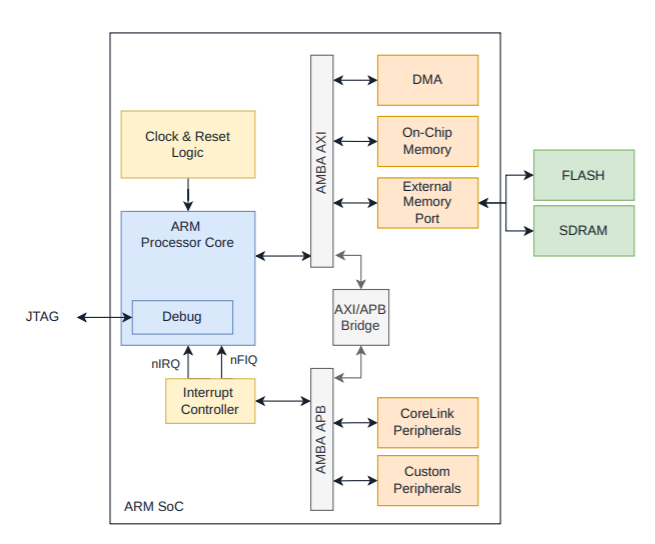
\includegraphics[width=.75\textwidth]{img/arm_internals.png}
    \caption{Architettura interna SoC}
    \label{img:ARM_internals}
\end{figure}

L'architettura presentata è generale ed è comunque molto flessibile: ogni azienda produttrice la personalizza in base alle proprie esigenze e alle mansioni per cui il sistema è dedicato.
Distinguiamo immediatamente tre famiglie di CPU ARM:
\begin{itemize}
    \item \textbf{ARM CORTEX A} - fascia ad alte prestazioni, orientata ad applicazioni general purpose;
    \item \textbf{ARM CORTEX R} - CPU pensate specificamente per supportare applicazioni time critical;
    \item \textbf{ARM CORTEX M} - CPU pensate per sistemi embedded come i microcontrollori.
\end{itemize} 

\uppercase{è} importante insistere sulla differenza tra architettura di un processore e implementazione di un processore che supporti tale architettura: L'\textbf{architettura} definisce un modello di programmazione, un insieme di registri, un insieme di istruzioni e un modello per la gestione delle interruzioni/eccezioni; L'\textbf{implementazione} invece è la realizzazione particolare di una determinata architettura (ARM-A8 e ARM-A9 sono entrambe implementazioni dell'architettura ARMv7-A, ma presentano dettagli realizzativi della pipeline diversi, pur presentando lo stesso set di istruzioni).

